\documentclass[
reprint,
amsmath,
amssymb,
aps,
%pra,
prl
%rmp,
%prstab,
%prstper,
%floatfix,
]{revtex4-1}
\usepackage{ctex}
\usepackage{graphicx}% Include figure files
\usepackage{dcolumn}% Align table columns on decimal point
\usepackage{bm}% bold math
\usepackage{subfigure}
% \usepackage{hyperref}% add hypertext capabilities
\newcommand{\RomanNumeralCaps}[1]{\MakeUppercase{\romannumeral #1}}
\makeatother

\begin{document}
\title{布朗运动与DNA 随机行走}
  \author{SA18002024  吴双祥}
  \affiliation{中国科学技术大学物理学院}%
  \date{\today}

  \begin{abstract}
    参考文献《布朗运动100年》,本文首先简要介绍一下扩散方程与随机行走在数学上的联系。
    接着采用数值模拟的方法来详细说明这一点。
    然后介绍了 “DNA 随机行走” 这样一种用来研究基因的某种统计学方法。
    简要说明了一些相关的参考文献有趣结果,试图重现其结果。
  \end{abstract}

  \maketitle

  \section{扩散方程与随机行走}%
  \label{sec:bu_lang_yun_dong_yu_sui_ji_xing_zou_}
  著名的扩散方程具有以下形式,
  \begin{equation} \label{eq:diffusion_eq}
  \frac{\partial \rho}{\partial t}=D \frac{\partial^{2} \rho}{\partial x^{2}}
  \end{equation}
 假定在 $t =0$ 时刻粒子位于 $x =0$ 处,即
 $\rho(x , 0) = \delta ( x )$,扩散方程的解是:
 \begin{equation} \label{eq:rho_xt}
  \rho(x, t)=\frac{1}{\sqrt{4 \pi D t}} e^{-\frac{x^{2}}{4 D t}},
 \end{equation}
 即粒子的密度遵从高斯分布。对于固定的时刻 $t$ 有,
 \begin{equation}\label{eq:x_mean_and_variance}
 \langle x\rangle= 0, \quad\left\langle x^{2}\right\rangle= 2 D t,
 \end{equation}
 可以验证 $\displaystyle{\int_{-\infty}^{\infty}\rho(x,t) \mathrm{d}\,t=1}$。
 这样就得到了扩散长度公式,
 \begin{equation} \label{eq:standard_deviation}
 \sqrt{\left\langle x^{2}\right\rangle}=\sqrt{2 D t},
 \end{equation}
 这里出现了著名的爱因斯坦的 $\frac{1} {2}$ 指数。
 
 另一方面,如果把时间离散化为步长为 $\delta t$ 的 小 段,令 $t = n \delta t$ ,同时保持 $\delta t$ 适当大,使得每小段时间头尾的运动彼此无关,于是行走 $n$ 步的结果 $x_n$ 就是 $n$ 个独立随机变量之和。
 那么显然地,随机行走的结果应该与上述扩散方程具有相同的行为,即有 $x_n$ 服从正态分布, 
\begin{equation} \label{eq:x_random_mean_variance}
	\left\langle x_{n}\right\rangle= 0,\left\langle x_{n}^{2}\right\rangle \propto n.
\end{equation}
 
 事实上,这个性质就是统计学中的中心极限定理的概念,下面来详细说明一下。
 
{\kaishu 设随机变量 $ X_{1},X_{2},\cdots ,X_{n}$ 独立同分布, 且具有有限的数学期望和方差 $E(X_{i})=\mu$, $D(X_{i})=\sigma ^{2}\neq 0(i=1,2,\cdots ,n)$。记 ${\bar {X}={ \frac {1}{n}}\sum _{i=1}^{n}X_{i}}$, $\zeta _{n}={\frac {{\bar {X}}-\mu }{\sigma /{\sqrt {n}}}}$,则 ${ \lim _{n\rightarrow \infty }P\left(\zeta _{n}\leq z\right)=\Phi \left(z\right)}$ .} 

此定理的证明可见于一般的统计学教程之中,这里不再赘述。
重要的是此定理指出了独立同分布的随机变量之和服从正态分布,无论该随机变量服从何种分布。
对于随机行走来说,走出的每一步可以认为是没有关联的,即行走步数是独立同分布的,因此 $n$ 步的和 $x_n$ 就满足正态分布,与扩散方程的结果相契合。

为了对此定理有更直观的理解,本文选取了一些独立同分布的随机变量,并求其和来验证是否服从正态分布,在此基础上看其均值和方差是否与式 (\ref{eq:x_random_mean_variance}) 相同。计算结果如图 \ref{fig:center_thm} 所示。可以看出来随机行走的距离与正态分布的曲线符合得十分好,此外,一些统计学的检验工具 (scipy.stats.normaltest) 也说明了其距离服从正态分布。
更进一步地,计算得到的距离的均值和方差也和式 (\ref{eq:x_random_mean_variance}) 相吻合,从而通过计算的角度验证了中心极限定理。

\begin{figure}
	\centering
	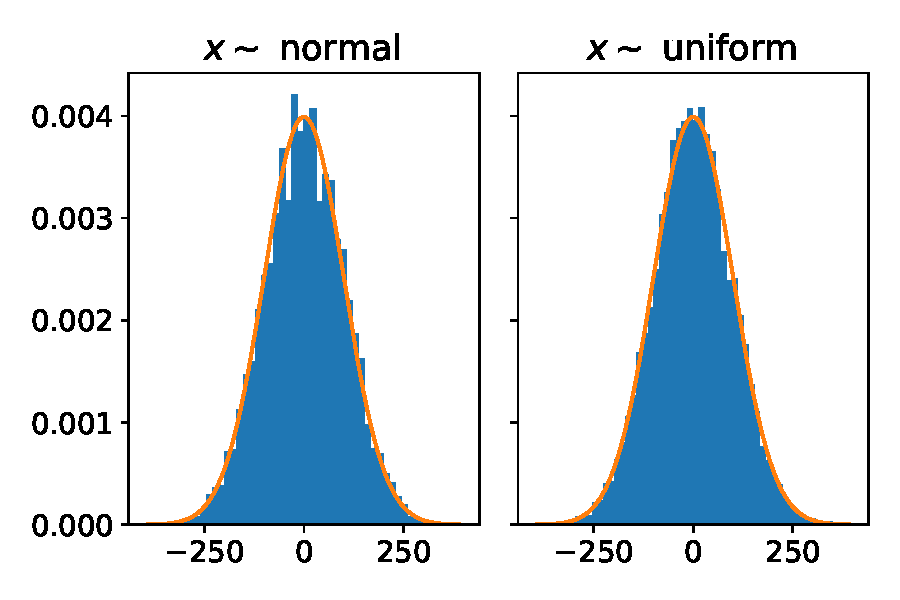
\includegraphics[width=\columnwidth]{center_thm.pdf}
	\caption{\label{fig:center_thm}通过数值模拟得到的随机行走分布图。左子图的随机变量 $x$ 服从正态分布,右子图的随机变量 $x$ 服从均匀分布。图中的橙色线条代表的是正态分布的曲线。}
\end{figure}

\section{DNA 随机行走}
在参考文献***中提到了将随机行走的概念应用至 DNA 链上来研究不同基因的碱基对的统计学性质。
有一种一维的随机行走研究方法是这样的:考察长度为 $n$ 的某一基因的碱基对序列,遇到嘌呤(A或者G)就向右走一步,遇到嘧啶(C或T)就向左走一步,最后检查这种随机行走到原点的方差 $\left\langle r_{n}^{2}\right\rangle$。
对于一般来说有 $\left\langle r_{n}^{2}\right\rangle \propto n^{\alpha}$,那么对于某一特定的 DNA 链,$\alpha$ 是大于、小于还是等于 $\frac{1}{2}$ 呢?
$\alpha$ 的取值也就代表了该基因的某种信息。

参考文献***给出了十分有意思的结果,说明了在
 \end{document}
